\section{Results}

Since the simulation contains non-deterministic processes and a steady state simulation is desired,
the time until a steady state is reached first had to be determined. Initially, this was attempted by running multiple
simulations with gradually increasing simulation time. The result can be seen in figure \ref{fig:steadyStateInitial}.
\begin{figure}[ht]
    \centering
    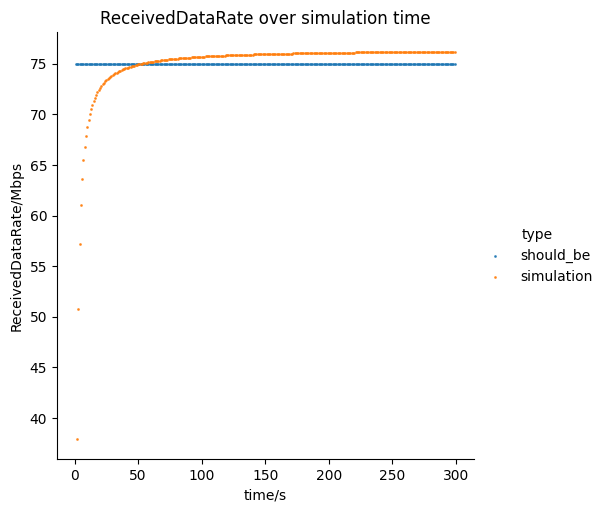
\includegraphics[width=0.4\textwidth]{../DataAnalysis/results/dr_over_time.png}
    \caption{average datarate over simulation duration}
    \label{fig:steadyStateInitial}
\end{figure}
However, this approach was deemed unrealistic. Upon plotting the data rate of a single simulation over time,
it was found that the data rate fluctuated heavily in the first 3 seconds and then stabilized.
This can be seen in figure \ref{fig:steadyStateInitialSingle}.

\begin{figure}[ht]
    \centering
    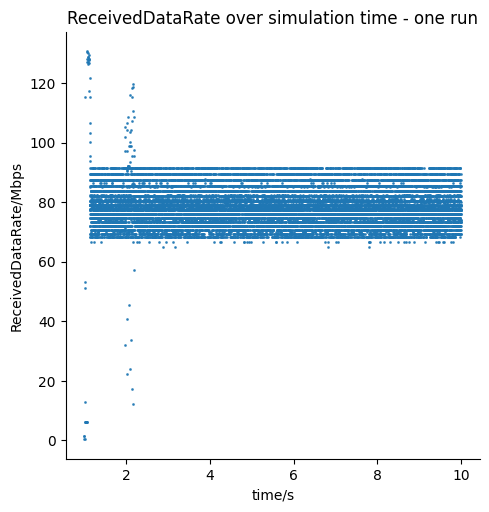
\includegraphics[width=0.4\textwidth]{../DataAnalysis/results/dr_over_time_single_run.png}
    \caption{datarate over simulation time of a single run}
    \label{fig:steadyStateInitialSingle}
\end{figure}

Keeping this in mind, the first graphic was redone, this time only using the data rate after 3 seconds for each simulation.
The result can be seen in figure \ref{fig:steadyStateFinal}.

\begin{figure}[ht]
    \centering
    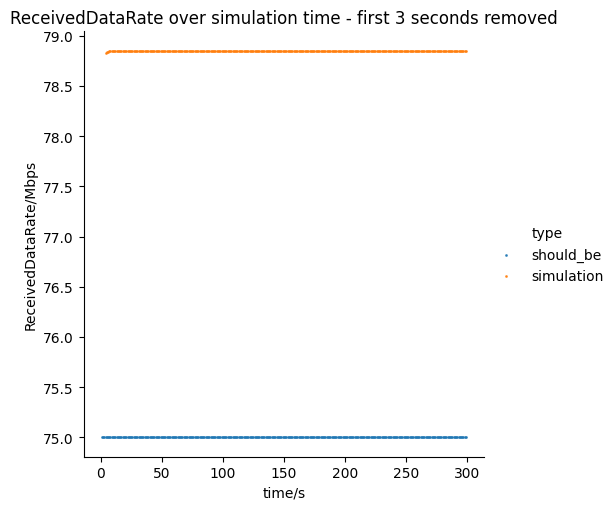
\includegraphics[width=0.4\textwidth]{../DataAnalysis/results/dr_over_time_without_first_3_seconds.png}
    \caption{average datarate over simulation duration without first 3 seconds}
    \label{fig:steadyStateFinal}
\end{figure}

It shows that the average data rate of a simulation is stable after 3 seconds and independent of how much longer the simulation 
time is running for - which in turn means the the datarate fluctuations seen in figure \ref{fig:steadyStateInitialSingle} can be assumed to be 
uniformly distributed. This means as long as the simulation time is long enough after the 3 seconds to reach a statistically relevant 
average value, the data rate can be assumed to be independent of the simulation time. With this information, it was 
decided to run the simulations for 10 seconds and only use the output after 3 seconds.

The same procedure was performed for the Rx power. The results of one run can be seen in figure \ref{fig:rxPowerSteadyState}.
\begin{figure}[ht]
    \centering
    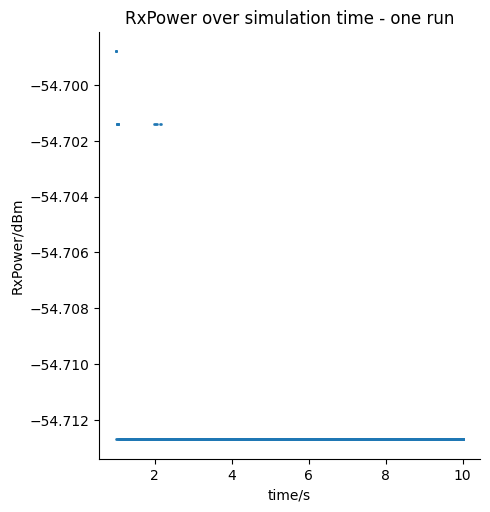
\includegraphics[width=0.4\textwidth]{../DataAnalysis/results/results_rx_pwr_over_time.png}
    \caption{Rx power over simulation duration}
    \label{fig:rxPowerSteadyState}
\end{figure}

For the Rx power, the fluctuations are much smaller. Therefore, it was decided to simply use the average Rx power over the
time of the simulation. This meant the averaging could be offloaded to the ns3 script, drastically 
reducing the computational load of the data analysis.

After determining the steady state, the simulations were run for 10 seconds of simulation time from a distance of 1 meter 
up to a distance where no more data arrived for each propagation model with a step size of 1 meter.

The results for the data rate can be seen in figure \ref{fig:drOverDistance}.
It shows that for the Friis- and the Two-Ray-Ground propagation model, the data is so similar that they are indistinguishable.
This was verified by plotting each of them separately to make sure each contains data, and then plotting them together. This plot only
shows informaion already contained in figure \ref{fig:drOverDistance} and is therefore not included in this report.
The results for Friis- Two-Ray-Ground- and ThreeLog-Distance propagation models also show 3 unexpexted exponential spikes
in the data rate between 50 and 100 meters. The reason for this should be  investigated in future work.
Apart from that, the three models show the expected behaviour. The rate plateaus at a HtMCS specified rate until a 
critical distance is reached, after which it first drops exponentially as packets increasingly fail to reach the receiver. 
This behaviour stops when the acceptable limit for packet loss is reached by the remote station manager, after which it 
switches to a more robust HtMCS and the data rate plateaus again. This happens until a maximum distance is reached, after which
no more packets arrive at the receiver. 
Both the Nagakami and Fixed Rss models stay fixed at a data rate of about 75 Mbps until the critical distance is reached,
at which point the data rate drops to close to 0. It actually never reaches 0, but stays at between 0.1 and 0.2 Mbps. Due to 
limits of the computational power available, the simulations were not run for long enough to reach find out at what distance
the data rate would actually reach 0. It did not at up to 4 km, and theoretically could reach over 200 km - 
although with a low throughput \cite{inproceedings}.  These two models were again smilar enough that they were
indistinguishable in the plot. Again, separate plots were made to verify that each contained data etc.
\begin{figure}[ht]
    \centering
    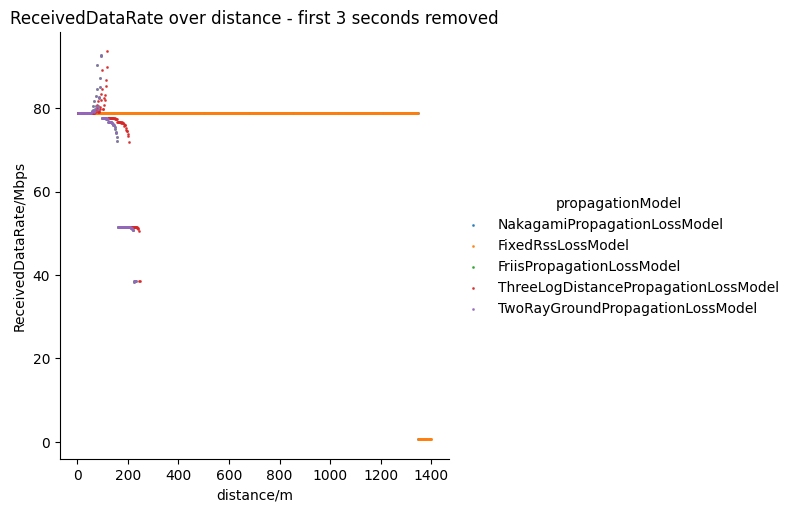
\includegraphics[width=0.4\textwidth]{../DataAnalysis/results/data_rate_comp.png}
    \caption{data rate over distance}
    \label{fig:drOverDistance}
\end{figure}

The results for the Rx power can be seen in figure \ref{fig:rxPowerOverDistance}.   
\begin{figure}[ht]
    \centering
    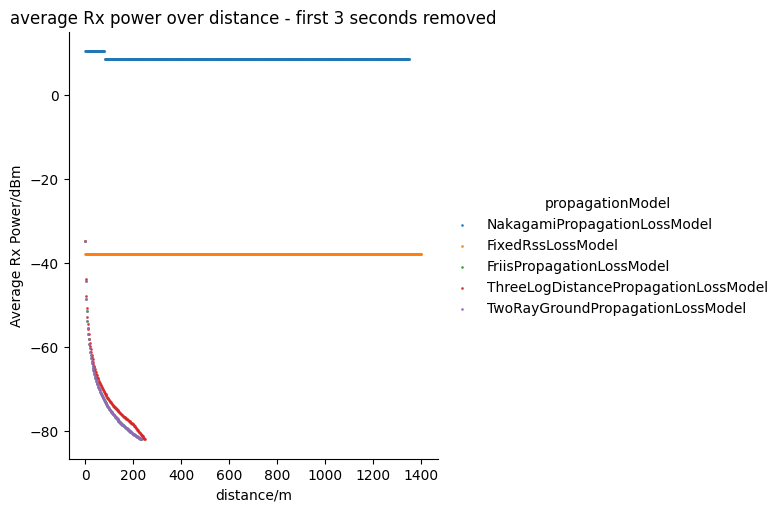
\includegraphics[width=0.4\textwidth]{../DataAnalysis/results/rx_pwr_comp.png}
    \caption{Rx power over distance}
    \label{fig:rxPowerOverDistance}
\end{figure}

The reason for the similarities between certain propagation models can be found in their configuration.
Since the default values for the propagation models (as of ns3 version 3.39) were used for all models, 
some of the models resulted in identical equations. Future work should investigate the differences between the models
with typical values for the parameters of each model.